\documentclass[12pt,fleqn]{article}\usepackage{../common}
\begin{document}
Kisitli Boltzmann Makinalari (Restricted Boltzmann Machines -RBM-)

Ikisel (binary) degerler tasiyan, gizli (hidden) $h$ degiskenler, ve yine
ikisel, gorunen (visible) degiskenler $v$ vardir. $Z$ aynen once gordugumuz
Boltzman Makinalarinda (BM) oldugu gibi normalizasyon sabitidir.

$$ p(x,h;W) = \exp (-E(x,h)) / Z $$

$$ E(x,h) = -h^TWx - c^Tx - b^Th $$

$$ = - \sum_j \sum_k W_{j,k}h_jx_k - \sum_k c_kx_k - \sum_j b_jh_j  $$

Dikkat: $h,x$ degiskenleri birer rasgele degiskendir. Yani hem $x$'e hem de
$h$'e ``zar attirabiliriz'', ya da bu degiskenlerden orneklem
toplayabiliriz. Bu kritik bir konu. 

Ustteki tanimlarda net sekilde goruluyor, ama bir daha vurgulayalim; gibi,
RBM'ler aynen BM'ler gibi bir olasilik dagilimidirlar. Yani tum mumkun
degerleri uzerinden entegralleri (ya da toplamlari) 1 olur, vs. 

RBM'lerin alttaki gibi resmedildigini gorebilirsiniz.

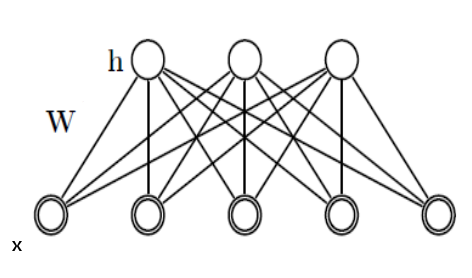
\includegraphics[height=4cm]{rbm_01.png}
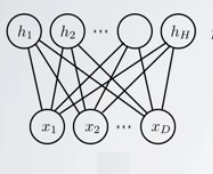
\includegraphics[height=4cm]{rbm_02.png}

RBM'lerin ``kisitli'' olarak tanimlanmalarinin sebebi gizli degiskenlerin
kendi aralarinda, ayni sekilde gorunen degiskenlerin kendi aralarinda direk
baglantiya izin verilmemis olmasidir, bu bakimdan
kisitlanmislardir. Baglantiya sadece gizli ve gorunen arasinda izin
verilmistir. Bu tabii ki matematiksel olarak bazi kolayliklar sagliyor.

Cebirsel olarak sunlar da dogrudur,

$$ p(x,h;W) = \exp (-E(x,h)) / Z $$

$$ = \exp (h^TWx + c^Tx + b^Th ) / Z $$

$$ = \exp (h^TWx) \exp (c^Tx) \exp(b^Th) / Z $$

Eger matris / vektor icindeki degerleri ayri degiskenler olarak gormek
istersek, 

$$ 
p(x,h;W) = \frac{1}{Z}
\prod_j \prod_k \exp (W_{jk}h_jx_k) \prod_k \exp(c_kx_k) \prod_j \exp(b_jh_j) 
 $$
















\end{document}
